\chapter{Grundlagen der Ökologischen Nachhaltigkeit}
Zuallererst bedarf es einer Definitition der ökologischen Nachhaltigkeit und weshalb diese überhaupt erstrebenswert ist. Die Wirtschaftsweise der Menschheit ist stehts im Wandel und unterscheidet sich von Land zu Land. Die immer gravierender werdenden Auswirkungen des menschengemachten Klimawandels haben dazu geführt, dass in den Köpfen der meisten Einwohner der Industrieländer Gier und die ``Geiz ist geil'' Mentalität lange nicht mehr attraktiv sind. Auch vor dem Hintergrund von Finanz- und Weltwirtschaftskrisen scheint die Motivation für einen grundlegenden wirtschaftlichen Wandel sogar größer denn je. Sei es Elektromobilität, vegetarische oder vegane Ernährung, Fair-Trade-Produkte, Kooperation mit Hilfsorganisationen oder Energiewende, alles soll heutzutage 'nachhaltig' sein, doch was genau ist überhaupt mit Nachhaltigkeit gemeint? \newline Der Begriff Nachhaltigkeit geht in seiner Verwendung auf den Freiberger Oberberghauptmann Carl von Carlowitz (1645-1714) und die Waldwirtschaft zurück\cite{doi:nachhaltig}. Der Kern der Aussage, in der der Begriff vorkam, war, dass laut Carlowitz in einem Wald nur so viel abeholzt werden sollte, dass dieser stets über die Kraft verfüge, auf natürliche Art und Weise nachzuwachsen. Es ging also um eine schlaue Art der Waldbewirtschaftung, die es kommenden Generationen ermöglichen sollte, ebenfalls von der kontinuierlichen Nutzung des Waldes zu profitieren. Die Definition, die bis heute am meisten Anwendung sowie Anerkennung findet und um welche es in dieser Arbeit gehen soll, ist also, dass Nachhaltigkeit generell als die Fähigkeit definiert wird, die Bedürfnisse der heutigen Generation zu befriedigen, ohne die Möglichkeiten künftiger Generationen zu gefährden, deren Bedürfnisse ebenfalls zu befriedigen. \clearpage Nun bleibt zu klären, in welche Felder die Nachhaltigkeit aus wirtschaftlicher Perspektive gegliedert wird. Aus Abbildung 2.1 lässt sich entnehmen, dass die Nachhaltigkeit sowohl sozialer, ökologischer als auch ökonomischer Natur sein kann, ich werde mich aber nur auf die Ökologie fokussieren.\newline Die Grundlage unserer Existenz besteht aus natürlichen Ressourcen. Ob veganes Sojaschnitzel, Klamotten oder unser geliebtes Smartphone, für alle Produkte wurden Wasser, Böden und Rohstoffe genutzt. Ohne diese natürlichen Ressourcen wären wir heute nicht, wer wir sind. Diese Ressourcen sind jedoch begrenzt, gerade Rohstoffe wie Erdöl und Metalle werden irgendwann aufgebraucht sein und können nicht grenzenlos zu Produkten verarbeitet werden. Das gleiche gilt für Ressourcen wie Sauerstoff und Energie. Genau diese Umstände, dass Menschen und ihr Konsum eine Auswirkumg auf die Gesamtumweltsituation haben, fällt unter den Begriff der Ökologie. 
Umgangssprachlich wird das Adjektiv ``ökologisch'' als Ausdruck für eine Haltung oder ein Agieren verwendet, das schonend mit Umweltressourcen umgeht\cite[13-23]{test123}. Wie diese ökologische Nachhaltigkeit durch moderne Technologien wie einer Blockchain-Anwendung erreicht und unterstützt werden kann, soll im folgenden prognostiziert werden.

\begin{figure}[ht!]
	\centering
	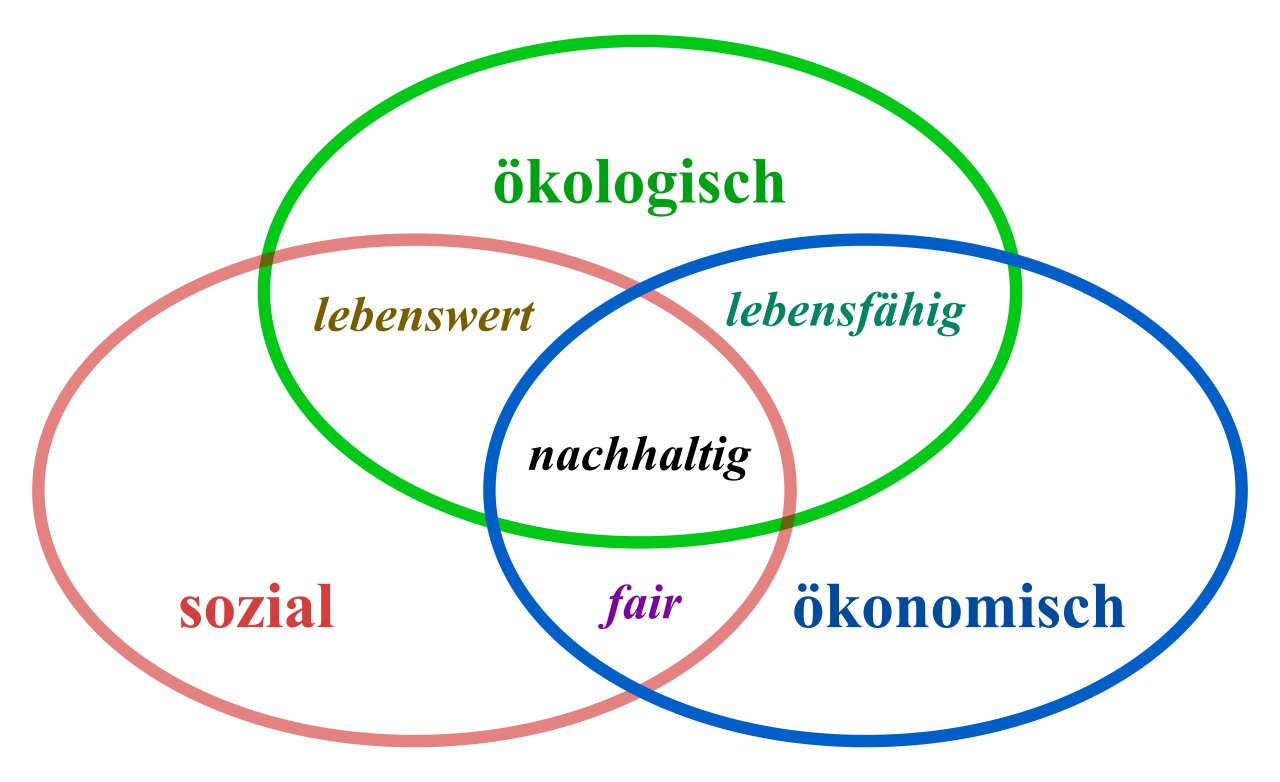
\includegraphics[width=100mm]{nachhaltig.jpg}
	\caption{Die drei Aspekte der Nachhaltigkeit\cite{oekologischeN} \label{overflow}}
\end{figure} 
\chapter{Technologische Grundlagen der Blockchain-Technologie}
\section{Mehr als nur Bitcoin}
\section{Zentral vs Dezentral}
Um das benötigte Verständnis zu schaffen, werde ich einige Grundlagen über Blockchain und Kryptowährungen klären und kurz erläutern, in welchem Zustand sich aktuelle Internetanwendungen befinden und wie diese in Zukunft aussehen könnten. \clearpage
Die ersten Computernetzwerke entstanden in den 1960er Jahren. Über die folgenden drei Jahrzehnte entwickelte sich das Netzwerk, welches unter dem Namen ARPANET vom Verteidigungsministerium der Vereinigten Staaten begründet wurde, zum Internet, das wir heute kennen und täglich verwenden\cite{arpanet}. Weitere 30 Jahre nachdem das Internet massentauglich wurde, bilden zentrale Datenarchitekturen immernoch die Grundpfeiler des gesamten Netzwerks. Das heißt, unsere Daten werden zentralisiert auf wenige Computer, welche als Server im Netzwerk Kopien jener Daten speichern und bereitstellen, damit sie von für uns Nutzer oder Clients stehts abrufbereit sind. Diese Praktik sollte Misstrauen hervorrufen, denn wenige, mächtige Institutionen sind somit in der Lage, wenn sie es denn wöllten, sehr effizient Daten zu manipulieren, zu löschen oder aber nur bestimmten Nutzern den Zugriff zu erlauben. Dafür müssten sie in den meisten Fällen nur genau einen Punkt im Netzwerk kontrollieren. Betrachtet man die ganze Welt, wird man schnell fündig, wie manche Regierungen von besagter Macht kurzerhand Gebrauch machen. 2017 hat die spanische Regierung genau diese Problematik ausgenutzt, um die Unabhängigkeit der Katalanen zu verhindern \cite{catalonia}.
\begin{figure}[ht!]
	\centering
	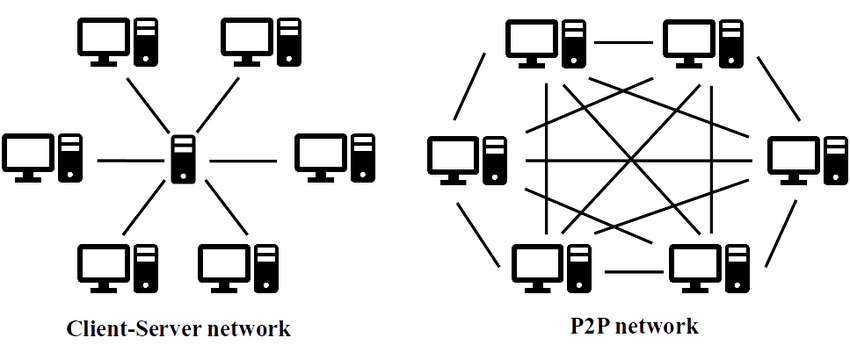
\includegraphics[width=100mm]{peer2peer.jpg}
	\caption{Vgl. Zentral vs. Dezentral\cite{p2p} \label{overflow}}
\end{figure}\newline Eine alternative Architektur ist die der Dezentralität. Diese dezentralen Anwendungen basieren auf sogenannten Peer-to-Peer-Netzwerken, in denen die Benutzer untereinander direkt kommunizieren und dies eben nicht über einen sich in der Mitte befindenden Server tun. Anwendungen dieser Art gibt es nicht erst seit 2009, dem Jahr in dem der Bitcoin vorgestellt wurde, aber mit ihm wurde ein neues Prinzip erfunden, das es anonymen Teilnehmern eines riesigen globalen Netzwerks ermöglicht, ein gegenseitiges Vertrauen zu schaffen, welches zuvor nur durch juristisch bindende Verträge oder zentrale Institutionen, also Banken oder Plattformen wie Google und Facebook, geschaffen werden konnte. Die Grundlage des Bitcoin-Protokolls ist, dass alle aktiven Teilnehmer, auch Nodes genannt, lokal eine Kopie des gemeinsamen Kursbuches (zu Deutsch ledger) abspeichern, wie es sonst nur von Banken geführt wird. In diesem Kursbuch stehen alle bisher getätigten Transaktionen seit Beginn des Bitcoins. Der Unterschied ist, dass in diesem Fall nicht ein zentraler Akteur eine einzige Kopie des Ledgers besitzt, sondern gleich alle Akteure weltweit Kopien mitführen. Es handelt sich also um ein verteiltes Kursbuch bzw im Englischen einen ``distributed ledger''. Das Bitcoin-Netzwerk wird auf den Händen dieser besagten Nodes getragen. Wollen diese Nodes aktiv neue Transaktionen ins Kursbuch hineinschreiben, so müssen sie im Bitcoin-Protokoll einen Beweis darüber vorzeigen, dass sie eine gewisse Rechenleistung erbracht haben, den sogenanngen Proof of Work. Hierdurch entsteht die Sicherheit des gesamten Netzwerks und auch dessen enorme Energielast, über welche in den Medien berichtet wird. Die verarbeiteten Transaktionen werden anschließend in Blöcke zusammengefasst und als Paket in das Kursbuch eingefügt. Es handelt sich also um eine immer länger werdende Kette aus Blöcken, daher der Begriff Blockchain. Für jeden Block, den ein Miner, also jemand der eine Node betreibt um neue Blöcke zu erstellen, an die Kette anfügt, wird er wiederum mit Bitcoins belohnt, damit ein Anreiz gegeben ist, eine horrende Stromrechnung in Kauf zu nehmen, um die Sicherheit des Bitcoin-Netzwerks zu unterstützen\cite{bitcoinWiki}. Genau hier liegt auch aktuell der ökologisch problematische Teil des ganzen Systems. Riesige Farmen, bestückt mit tausenden sogenannten ``Mining Rigs'', also hoch spezialisierten Computer-Chips, mit welchen man sehr effizient Bitcoin minen kann, bilden die Grundlage des Bitcoins. Größtenteils befinden sich diese natürlich in Ländern in dem der Strom sehr billig ist, zum Beispiel ´China, was bedeutet, dass ein großer Teil der Energie, welche benötigt wird um das Bitcoin-Netzwerk zu betreiben aus Kohlekraftwerken stammt, welche natürlich einen sehr miserablen Kohlenstoffdioxid Fußabdruck besitzen\cite{miningChina}\cite{bitcoin}.
\section{Smart Contracts}
test test test\cite{tesla}
\section{Konsensalgorithmus}
\chapter{Chancen und Risiken}
\section{Risiko 1 }
\section{Risiko 2}
\section{Lieferketten Transparenz}
Transparenz ist ein Begriff, der immer mehr an Bedeutung gewinnt. Gerade entlang der Liefer-und Versorgungskette von Konsumgütern würde eine Erhöhung der Transparenz eine Menge von Vorteilen bringen. Der Endverbraucher hat aktuell kaum eine Chance festzustellen, ob Dinge wie Umweltverschmutzung, Betrug oder gar Menschenrechtsverletzungen entlang der Produktionskette des Produktes entstehen, welches er vor sich im Supermarktregal sieht, denn auf die Verpackung passt einfach nicht genügend Information. Nichtsdestotrotz kommt es immer wieder vor, dass solche Negativumstände, nachdem viele Menschen ein Produkt gekauft haben, ans Licht kommen. Dies macht es sowohl Privatpersonen als auch Firmen schwer, nachhaltige Konsumentscheidungen zu treffen. In den aktuell verwendeten Systemen fehlen die Mittel zur verlässlichen Überprüfung von Verhalten entlang der Lieferkette. Die zuvor beschriebenen dezentralen Anwendungen, welche über Smart-Contracts auf einer grünen Blockchain laufen könnten, erzeugen hier Hoffnung, denn mit ihnen ist es möglich, ein bisher unerreichtes Niveau an Transparenz zu schaffen. Durch die Eigenschaft der transparenten Abspeicherung und der Unveränderbarkeit der dezentral abgelegten Daten wird es für Teilnehmer, fast unmöglich nachträglich falsche Fakten zu schaffen, sofern die Informationen welche ursprünglich eingespeist worden sind denn der Wahrheit entsprechen. Lieferketten sind also ein gutes Beispiel, anhand dessen man aufzeigen kann wie Blockchain-Lösungen die Nachhaltigkeit fördern könnten. Eine Lieferkette ist ein komplexes Netzwerk, das aus seperaten und räumlich voneinander getrennten Institutionen besteht. Diese Instituitonen wiederum befinden sich im ständigen Austausch von Produkten, Zahlungen und Daten. Blockhain-Anwendungen könnten hier ansetzen, um die Herkunft von Gütern und Dienstleistungen entlang der Kette nachvollziehbarer zu machen. Der zuvor erwähnte Austausch von zentraler durch dezentrale Blockchain-Architekturen kann auch hier enorme Vorteile bringen. Beispielsweise könnten Datenredundanzen und Dateninkonsistenzen, welche durch multiple Dokumentenkopien entstehen, vermieden werden, indem nur eine Version eines Dokuments im Blockchain-Kursbuch vermerkt wird. Auf Dauer kann hierdurch eine Echtzeit-Transparenz entlang der Lieferkette erreicht werden, sofern alle Teilnehmer software auf der Blockchain basieren und unter der Voraussetzung, dass die Blockchain-Lösungen durch Big Data und das Internet der Dinge (IoT) verknüpft werden. Denn ein wichtiger Aspekt ist, dass man den Daten, welche in die dezentralen Anwendungen gespeist werden, von Beginn an vertrauen kann, und dass dadurch IoT-Lösungen unverfälschte Echtwelt-Daten liefern.\newline
Die Herkunft von Gütern und Dienstleistungen ist ein Beispiel für Information welche transparenter kommuniziert werden kann. Wenn Güter ihre Endstation erreichen, wissen die meisten Käufer und Verkäufer nichts über den wahren Ursprung der hergestellten Ware oder über deren Inhaltsstoffe bescheid. Würde man als Verbraucher zum Zeitpunkt des Kaufs mehr Informationen erhalten, so hätte man deutlich mehr Möglichkeiten, aber auch mehr Verantwortung, über die Produktonsweise und Herkunft diverser Güter mitzubestimmen. Man könnte sich ein deutlich besseres Bild darüber machen ob das Gut umweltbelastend produziert worden ist und unter welchen Bedingungen dies geschehen ist. \newline Ein weiteres Beispiel ist die Nachvollziehbarkeit des Preises, denn mangelt es an ihr sowie an der Nachvollziehbarkeit der Kosten, die durch etwaige Zwischenhändler aufgeschlagen werden, so werden Endkonsumenten erheblich daran gehindert zu verstehen, wer welche Einnahmen in einer Lieferkette verzeichnen kann, oder auch, wie die Arbeitsbedingungen für die Produzenten sind\cite{lieferkette}.\newline Auch vor Plagiaten kann diese erhöhte Transparenz schützen. Mehr gesicherte Informationen machen es schwieriger, den Kunden von der Echtheit des gefälschten Produkts zu überzeugen. Auch dies würde die ökologische Nachhaltigkeit fördern, denn meist werden Plagiate unter umweltverschmutzenden Bedingungen mit minderer Qualität der Ressourcen geschaffen.\newline Eine Blockchain, die sich nur mit der Transparenz von Lieferketten beschäftigt und Anwendungen unterstützt, die man schon heute schon ausserhalb Deutschlands im alltäglichen Gebrauch finden kann, ist VeChain. Produkte, welche durch VeChain-basierte Anwendungen transparenter gestaltet werden, verfügen über einen NFC-Chip, welcher auf der Verpackung klebt. Öffnet man die Verpackung, geht der NFC-Chip kaputt, was dem Endverbraucher garantiert, dass der Inhalt unverändert die Fabrik verlassen hat. Scannt der Kunde den Chip mit seinem Handy, so erhält er ausführliche Informationen über das Produkt, welchen er mehr vertrauen kann als einem gedruckten Werbespruch auf der Verpackung oder einem vermeintlich glaubwürdigen Klimasiegel \cite{vechain}\cite{veDoc}.
\section{Chance 2}

